One goal of the {\sc Cleo III} resonance program is to measure
$\Gamma_{ee}$ (leptonic decay width) of $\Upsilon(1S)$,
$\Upsilon(2S)$, and $\Upsilon(3S)$ to high precision ($\sim$2\%).

This measurement takes advantage of a relation between $\Gamma_{ee}$
and the total hadronic yield of each resonance.  The beam energy was
scanned over the resonances, giving hadronic cross section as a
function of energy, which can be fit to obtain the area and hence
$\Gamma_{ee}$.

These are the primary backgrounds to $e^+ e^- \to \Upsilon(nS) \to
\mbox{hadrons}$.

\vfill

\begin{minipage}{6in}
\begin{center}
\huge \fbox{Sources of Background}
\end{center}

\vspace{0.25cm}
\hspace{-0.25cm}
\begin{center}
  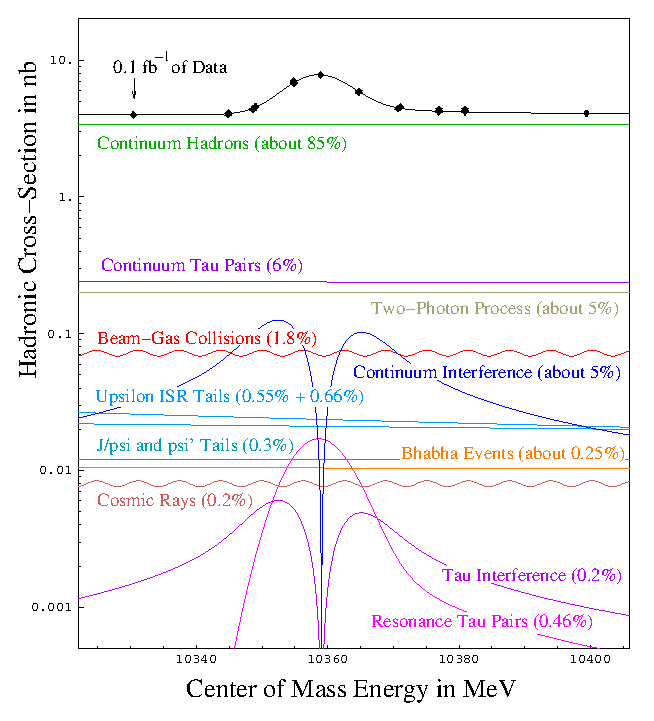
\includegraphics[width=\linewidth]{pivarski1.eps}
\end{center}

\end{minipage}

\newpage

Statistical uncertainties are small compared to the systematics, but
only the systematics due to backgrounds have been studied in detail.
The largest, interference between $e^+ e^- \to \Upsilon(nS) \to
q\bar{q}$ and continuum $e^+ e^- \to q\bar{q}$, is conservatively
estimated here.

The other primary sources of systematic error, stability of the energy
measurement and uncertainty in acceptance and luminosity, are either
bounded or conservatively estimated.

\vfill

\begin{minipage}{6in}
\begin{center}
\huge \fbox{Table of All Uncertainties}
\end{center}
\large

\vspace{0.25cm}

\hspace{-0.2cm} \begin{minipage}{\linewidth}
  \begin{tabular}{p{4.5cm} c c c}
    & {\LARGE $\Upsilon(1S)$} & {\LARGE $\Upsilon(2S)$} & {\LARGE $\Upsilon(3S)$} \vspace{0.25cm} \\

    \mbox{\LARGE Contribution to Uncertainty in yield (and $\Gamma_{ee}$):} & & & \vspace{0.2cm} \\
    Beam-gas & 0.04\% & 0.02\% & 0.05\% \vspace{0.1cm} \\
    Beam-wall & zero & zero & zero \vspace{0.1cm} \\
    Cosmic Rays & 0.003\% & 0.001\% & 0.003\% \vspace{0.1cm} \\
    Two-Photon Process & 0.02\% & 0.04\% & 0.03\% \vspace{0.1cm} \\
    $J/\psi$ and $\Upsilon$ ISR tails & 0.0006\% & 0.05\% & 0.03\% \vspace{0.1cm} \\
    $\Upsilon \to \tau^+ \tau^-$ & 0.02\% & 0.07\% & 0.04\% \vspace{0.1cm} \\
    \raggedright $e^+ e^- \to \tau^+ \tau^-$ \mbox{\hspace{0.65cm} interference} & 0.09\% & 0.08\% & 0.04\% \vspace{0.1cm} \\
    \raggedright $e^+ e^- \to q\bar{q}$ \mbox{\hspace{0.65cm} interference} & $\sim$0.3\% & $\sim$0.3\% & $\sim$0.3\% \vspace{0.1cm} \\\hline
    \mbox{\hspace{-0.1cm}
\includegraphics[width=15.5cm]{pivarski2.eps}} & & & \vspace{-0.85cm} \vspace{0.1cm} \\
    Sum of Backgrounds: & 0.32\% & 0.33\% & 0.31\% \vspace{0.5cm} \vspace{0.1cm} \\

    Statistics & 0.13\% & 0.30\% & 0.48\% \vspace{0.5cm} \vspace{0.1cm} \\

    \mbox{\LARGE {\it Predicted} Contributions:} & & & \vspace{0.2cm} \vspace{0.1cm} \\
    Energy Stability & $<$ 0.6\% & $<$ 1.0\% & $<$ 0.9\% \vspace{0.1cm} \\
    Acceptance & $\sim$ 0.6\% & $\sim$ 0.6\% & $\sim$ 0.6\% \vspace{0.1cm} \\
    Luminosity & $\sim$ 2\% & $\sim$ 2\% & $\sim$ 2\% \vspace{0.25cm} \vspace{0.1cm} \\\hline
    & & & \vspace{-0.35cm} \vspace{0.1cm} \\

    \mbox{\hspace{-0.1cm}
\includegraphics[width=15.5cm]{pivarski3.eps}} & & & \vspace{-0.9cm} \vspace{0.1cm} \\
    \mbox{\LARGE Predicted Totals:} & \mbox{2.2\%} & \mbox{2.4\%} & \mbox{2.3\%} \vspace{0.5cm} \vspace{0.1cm} \\

    PDG Best Value
    & \hspace{1.15cm} 3.3\% {\small ({\sc Novo} '96)} \hspace{-0.90cm} 
    & \hspace{1.15cm} 6.4\% {\small ({\sc Novo} '96)} \hspace{-0.90cm} 
    & \hspace{1.15cm} 9.4\% {\small ({\sc Cleo} '84)} \hspace{-0.90cm} \vspace{0.1cm} \\
    PDG Average & 2.2\% & 4.1\% & 9.4\% \\

  \end{tabular}
\end{minipage}

\end{minipage}

\newpage

